\section{Test cases} \label{sec:tests}

The following is a tentative list of test cases for the algorithm.
\begin{enumerate}
\item A moving box in a fixed pressure field. No FSI, but testing
of several components in the program.
\item A beam mounted perpendicular to the flow. The beam is fixed to
the floor at one end and free to move at the other.
\item An elastic hydrofoil with varying angle of attack, \cite{DY:1}.
\item A propeller blade in a varying inflow.
\item A hull structure excited by non-steady propulsion force.
\end{enumerate}

The beam test case is fundamental for the verification of the
algorithm and the implementation, and several tests should be
performed for the beam. Apart from cross-flow, the beam should
be tested in a still fluid, to check the change in oscillation
frequency due to the added mass of the surrounding fluid.
When started in cross-flow, the beam should first bend in the flow
direction and then, when vortex shedding starts, it should go
over to oscillations in the transversal direction.

%--------------------------------------------
%
%     M O V I N G   B O X
%
\subsection{The moving box}

This test case does not contain fluid-structure interaction but
is designed to only check the following parts of the implementation.
\begin{itemize}
\item Input and output concerning the structural mode description.
\item Construction of the right hand side in the ODE for the mode coefficients.
\item Solution of the ODE for the mode coefficients.
\end{itemize}

The geometry is a rectangular box inside a cube.
The sides of the boxes are aligned with the coordinate directions.
The outer box is stationary and the inner
box can move as a rigid body along the coordinate axes.
The geometrical parameters of the problem are given in table~\ref{tab:boxParam}.
The motion of the body is driven by a prescribed pressure field which is contant
in time and is given by the expression,
\[
p=\left\{\begin{array}{lll}
\Delta p & \mbox{for} & x>0.5 \\
0 & \mbox{for} & x \leq 0.5
\end{array}\right.
\]
The pressure jump, $\Delta p$, and other physical parameters are given in
table~\ref{tab:boxPar}, and the pressure distribution is illustrated in 
figure~\ref{fig:boxP}.

\begin{figure}
\centering
\caption{The pressure distribution for the moving box test case, on the plane~$z=0$.}
\label{fig:boxP}
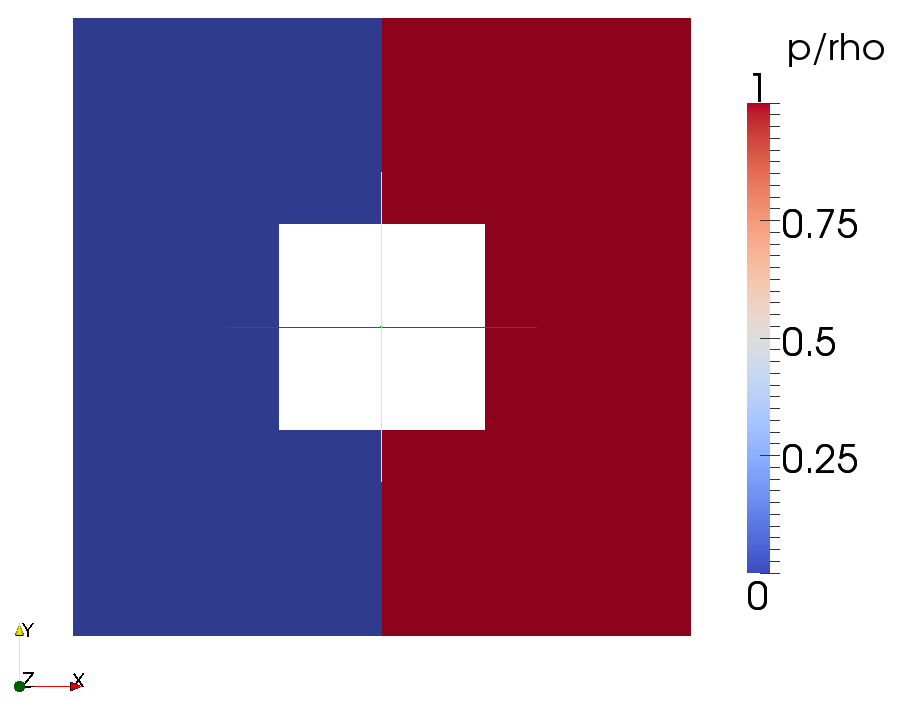
\includegraphics[width=0.7\linewidth]{figures/ml/fig1}
\end{figure}


\begin{table}[htp!]
\centering
\caption{The dimensions of the outer and inner boxes. All quantities
are given in meters, square meters or cubic meters as appropriate.}
\label{tab:boxParam}
\begin{tabular}{c|cc|}
&  Outer box & Inner box  \\ \hline
$x_{min}$ & 0  & $1/3\approx 0.3333$  \\
$x_{max}$ & 1  & $2/3\approx 0.6667$  \\
$y_{min}$ & 0  & $1/3\approx 0.3333$  \\
$y_{max}$ & 1  & $2/3\approx 0.6667$  \\
$z_{min}$ & 0  & $3/7\approx 0.4286$  \\
$z_{max}$ & 1  & $4/7\approx 0.5714$  \\ \hline 
$V$  & 1 & $1/63\approx 0.0159$ \\
$A_x=A_y$ & 1 & $1/21\approx 0.0476$ \\
$A_z$ & 1 & $1/9\approx 0.1111$ \\  \hline
\end{tabular}
\end{table}

\begin{table}[htp!]
\centering
\caption{Physical parameters. Note that the solid density can be calculated
from the prescribed modal functions, as described in the text.}
\label{tab:boxPar}
\begin{tabular}{l|ccc|}
Quantity & Notation & Value & Unit \\ \hline
Fluid density & $\rho_f$ & 1000 & kg/m$^3$ \\
Pressure jump & $\Delta p$ & 1000 & Pa \\ \hline
\end{tabular}
\end{table}


The modal motion of the box is represented by three modes with the
frequencies,
\[
f_1=1\,\mbox{Hz},\hspace{1cm}
f_2=2\,\mbox{Hz},\hspace{1cm}
f_3=3\,\mbox{Hz},
\]
and mode shapes corresponding to rigid body motion in the three coordinate directions,
\[
\bphi_1(\bx)=a \be_x\hspace{1cm}
\bphi_2(\bx)=a \be_y\hspace{1cm}
\bphi_3(\bx)=a \be_z,
\]
where, $a=0.1\,$m.


The only way that the solid density enters the algorithm is through the normalization
of the modes. Given the information above, we can thus calculate which structural
density, $\rho_s$, it corresponds to.
\[
1=\int_{V_s}\rho_s|\bphi(\bx)|^2\,\mbox{d}V=\rho_s V_i\cdot a^{2}
\]
Using this expression and the inner box volume given in table~\ref{tab:boxParam},
we obtain, $\rho_s=6300\,$kg/m$^3$.

For this case, the forcing integrals can be evaluated analytically. For the first mode,
we have,
\[
Q_1=-\int_S p\bn\cdot \bphi_i\,\mbox{d}S=-\Delta p A_x a \approx -4.76 \mbox{Nm}.
\]
For the second and third modes, the forcing is zero, $Q_2=Q_3=0$.

\subsubsection{Analytical solution of first mode motion}

The motion of the block can thus be calculated by the solution of the ODE
for the first mode coefficient,
\[
\frac{\mbox{d}^2\alpha_1}{\mbox{d}t^2}+
\omega_1^2\alpha_1=Q_1,
\]
with inital data,
\[
\alpha_1(0)=0, \hspace{1cm} \dot{\alpha}(0)=0.
\]
The solution is given by the following convolution expression, for a general
time dependent forcing $Q_1(t)$, which then can be simplified since in the present case,
the forcing is constant.
\[
\alpha_1(t)=\frac{1}{\omega_1}\int_0^t \sin\left[
\omega_1(t-\tau)
\right] Q_1(\tau)\,\mbox{d}\tau=
\frac{Q_1}{\omega_1^2}(1-\cos \omega_1t)
\]

\subsubsection{Computed motion of the first mode}

The problem is solved by a program which involves all the functionality related to
the structural motion, but without the fluid solver. As described above, only
a pressure field (constant in time) is provided, which drives the structural motion.
Now we describe how input is provided to the program.

\vspace{0.2cm}

\noindent 1. The modes are described in the file:

\texttt{constant/structuralModes/modeData\_movingBlock}

\noindent Here is a segment of this input file relating to the first mode:

------------------------------

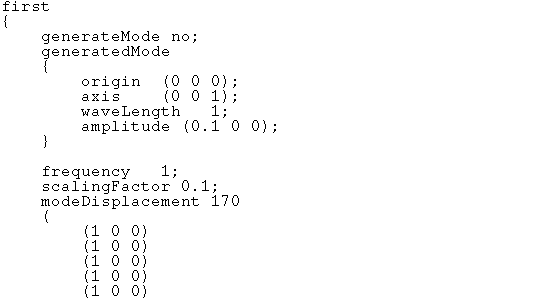
\includegraphics[width=0.7\linewidth]{figures/ml/data1}

------------------------------

\vspace{0.2cm}

\noindent 2. The input to the mesh deformation is given in the file:

\texttt{constant/dynamicMeshDict}

\noindent This file contains the following information:

------------------------------

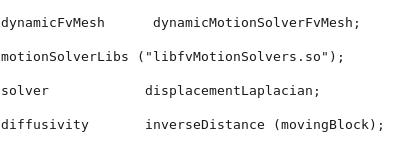
\includegraphics[width=0.55\linewidth]{figures/ml/data2}

------------------------------

\vspace{0.2cm}

\noindent 3. The remaining input, initial grid, pressure field, controls for time stepping etc,
are given in the same way as for a standard simulation case.
The case is simulated on the time interval, $0<t<10\,\mbox{s}$, with a time
step, $\Delta t = 0.01\,\mbox{s}$.

\begin{figure}[htbp!]
\centering
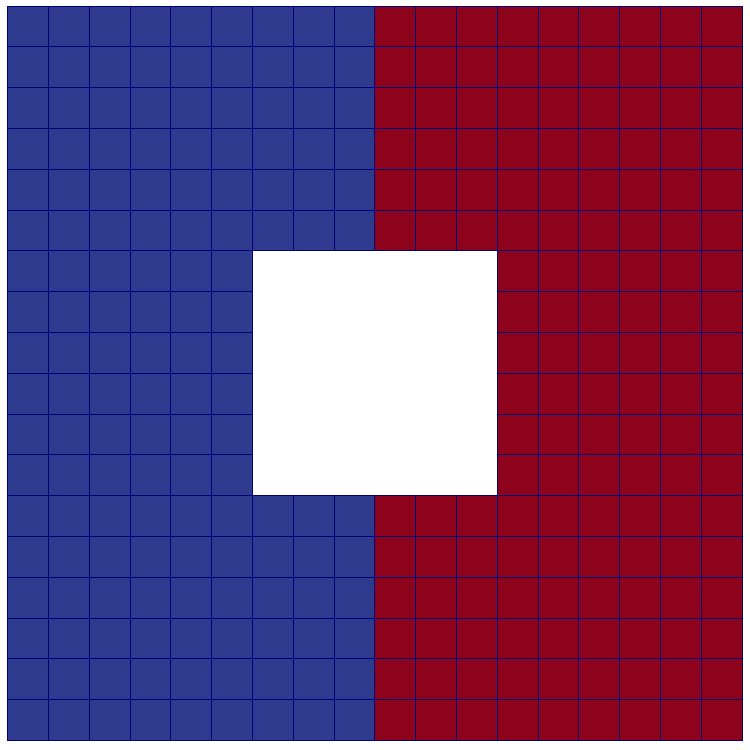
\includegraphics[width=0.4\linewidth]{figures/ml/noDef}
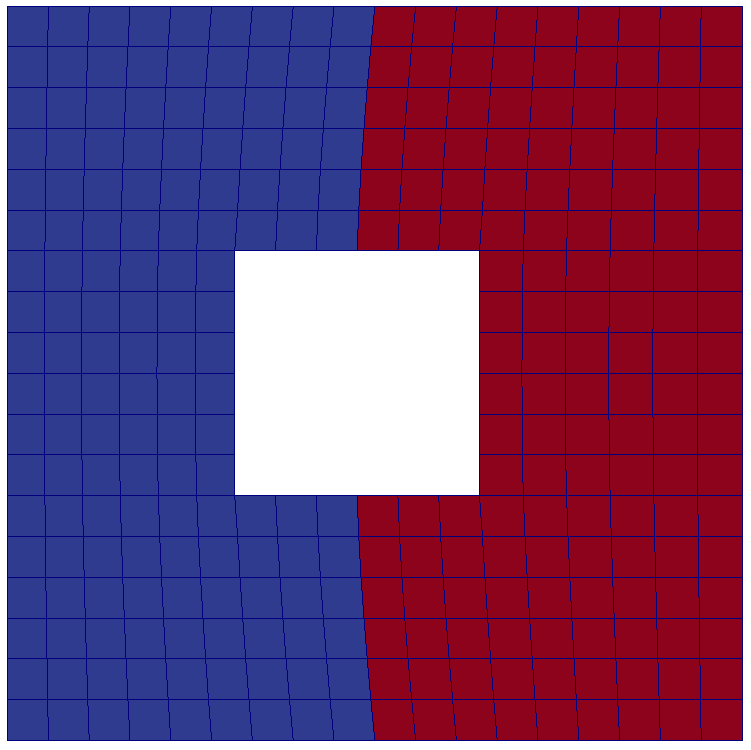
\includegraphics[width=0.4\linewidth]{figures/ml/maxDef}
\caption{Initial (undeformed) stat to the left, and maximal displacement, at $t=0.5\,$s,
to the right.}
\label{fig:boxDef}
\end{figure}

In figure~\ref{fig:boxDef}, we illustrate the grid deformation in the most deformed
state, at $t=0.5\,$s, and compare it to the initial grid.

\begin{figure}[htbp!]
\centering
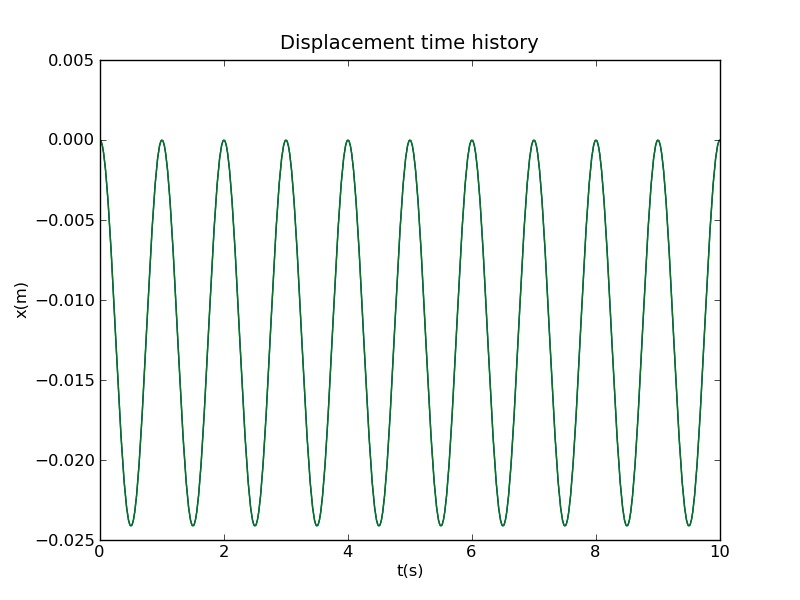
\includegraphics[width=0.49\linewidth]{figures/ml/displ.jpg}
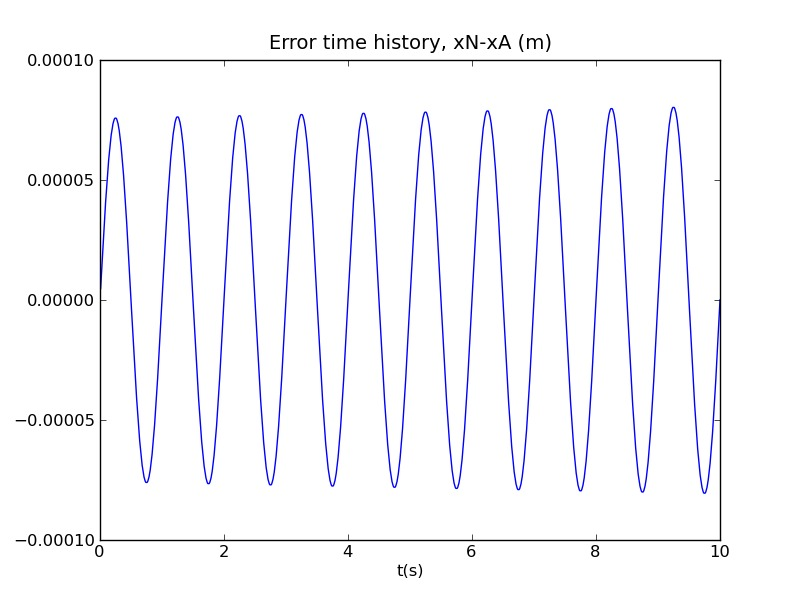
\includegraphics[width=0.49\linewidth]{figures/ml/diff.jpg}
\caption{Box displacement (in $x$-direction)
as function of time, $x_N(t)$, to the left, and error, $x_N(t)-x_A(t)$, to the right.}
\label{fig:displ}
\end{figure}

In order to check the computed motion, we post-process the computed displacement
for a point on the box. The displacement is only in the $x$-direction, and we
denote it by $x_N(t)$, where the sub-script indicates ``numerical''. We also
compare this to the exact analytical solution for the displacement, which we
denote $x_A(t)$. The displacement and the error are shown in figure~\ref{fig:displ}.
We note that the error is less than 0.34\% of the oscillation amplitude
over the whole simulation interval.

\subsection{The beam}

Cantilever beam = fixed at one end ...

The material parameters seem to correspond to something like rubber ...

\begin{table}[htbp!]
\centering
\caption{Material and geometrical parameters of the cantilever beam
with quadratic cross section and cross-sectional area $D^2$.}
\begin{tabular}{l|ccc|}
Quantity & Notation & Value & Unit \\ \hline
Modulus of elasticiy & $E$ & 0.03 & GPa \\
Poisson's ratio & $\nu_s$ & 0.3 & - - - \\
Density & $\rho_s$ & 5000 & kg/m$^3$ \\ \hline
Length & $L$ & 0.1 & m \\
Width & $D$ & 0.02 & m \\ \hline
\end{tabular}
\end{table}

\subsubsection{Mode generation, interpolation to CFD and scaling}

Two modal analyses are performed in two softwares. Comsol Multiphysics and
Ansys.  Both softwares delivered the same mode shapes, but the mode
normalisation was only successfully made in Ansys. The latter has as default
normalisation option to scale the modes with the \emph{mass matrix}, which
turns out to comply with the above equation \ref{eq:volint}, as discussed
below.

Mode data are exported from the structural solver as displacement vectors at
each solid mesh point, in ascii column data file format, where each row
contains point coordinates and corresponding displacement. This data then be
interpolated to the CFD boundary using the implemented OpenFOAM utility
\texttt{interpolateModeData}. In short, this utility reads a set of "mode
files" exported from the structural solver, and writes their interpolated
counterparts to another set of files. The latter is then included in the
dictionary defining the modes to be included in the OpenFOAM FSI.

To be able to assert that each mode fulfills equation \ref{eq:volint},
another utility is written: \texttt{calculateModeScaleFactor}. This
utility requires the same dictionary input as the FSI case, but must
be run on the solid itself. That is, a mesh in the solid region needs
to be generated. In the case of the cantilever beam, this is trivial.

When mode data for the first five modes from Ansys are interpolated to the
OpenFOAM case consisting of the solid beam, \texttt{calculateModeScaleFactor}
is run on each of the modes and the result is assuring: For all bending modes
the scale factor calculated by the OpenFOAM utility is very close to unity.
The exception is the third torsion mode, for which the scale factor seem to
be more difficult to calculate based on displacements in a cartesian system.

To conclude: Modes exported from a structural solver can be interpolated
to the OpenFOAM case and in case the normalisation of these modes is believed
to disagree with equation \ref{eq:volint}, the scale factor can be calculated
using an OpenFOAM case consisting of the solid only.
